% !TeX root = ../main.tex

\chapter{关键技术}

本章节将逐一介绍构建实时三维重建及语义分割系统所需的关键技术,从相机位姿估计到深度学习模型,再到并行计算和图形渲染技术,为后续系统的设计与实现奠定理论与技术基础。

\section{基于对极几何算法的相机位姿估计}

\par 对极几何是计算机视觉和立体视觉领域的一个基本概念,它描述了两个相机之间的基本几何关系,
可以用来表示三维空间中的某个点在两张图像上的投影点之间的几何约束关系。

\begin{figure}[htb]
	\centering
	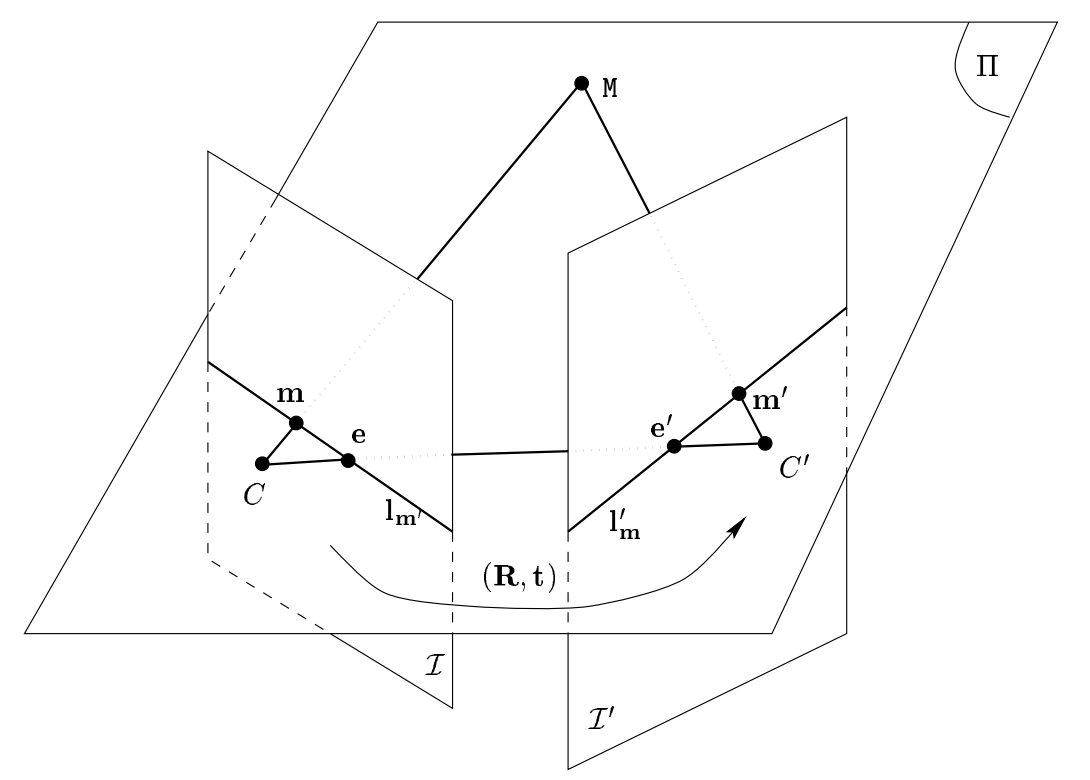
\includegraphics[width=0.7\textwidth]{figures/epipolar.png}
	\caption{对极几何示意图}
	\note{注:两个相机从不同位置观察同一三维点时,形成的对极平面、对极线以及基线。}
	\label{fig:epipolar}
\end{figure}

\par 如图\ref{fig:epipolar}\cite{epipolar}所示,有两个相机,一个在位置$C$,另一个在位置$C'$。它们都观察到了
同一个三维点$M$。$C$和$M$之间的连线与$C'$和$M$之间的连线交于$C$和$C'$之间的连线,这条线
称为基线(Baseline)。现在,可以在两个相机的图像平面上找到与$M$对应的两个二维点$m$
和$m'$。$m$,$m'$,$C$和$C'$共面,这个平面被称为对极平面(epipolar plane)。对极平面与
图像平面的交线被称为对极线(Epipolar Line),这条线包含了三维点$M$可能在图像上投影的所有位
置。这就是对极约束(Epipolar Constraint)。

\par 对极几何为估计相机的位姿提供了理论基础。利用它可以估计两个相机之间的相对位姿,
这是重建三维场景的关键步骤。利用对极约束,可以通过以下公式来估计相机的位姿:
\begin{equation}
	m'^T F m = 0
\end{equation}
\par 其中,$F$是基本矩阵(Fundamental Matrix),它封装了两个相机之间的相对位姿,$m$和$m'$是
对应的图像点。可以通过八点法或者随机采样一致性算法(Random Sample Consensus,RANSAC)等方法求解。一旦计算出$F$,就可以通过奇异值分解
(Singular Value Decomposition,SVD)来恢复旋转矩阵$R$和平移向量$t$:
\begin{align}
	F     & = K'^{-T} [t]_x R K^{-1} \\
	[t]_x & =
	\begin{bmatrix}
		0    & -t_z & t_y  \\
		t_z  & 0    & -t_x \\
		-t_y & t_x  & 0
	\end{bmatrix}
\end{align}
\par 其中,$K$和$K'$是相机的内参矩阵,$[t]_x$是$t$的反对称矩阵。
\par 最后,可以通过三角测量(Triangulation)恢复三维点$M$的坐标。

% \par 以上公式对应的是理想情况。然而,在实际应用中,需要考虑噪声和误差。因此,通常会使用
% 优化方法,比如使用最小二乘法(Least Squares)或者 Bundle Adjustment 来精细化位姿估计和
% 三维点的坐标。

% \par 对极几何是摄像机位姿估计的基础,然而它也有自身的局限性,比如不能处理在单一视图中的
% 旋转,即单应性问题。面对这个问题,可以使用比对极几何更具有普遍性的几何模型——多视几何(multiview
% geometry)。

% \par 多视几何可以处理三个或更多的视图,从而利用更多的信息来提高重建的质量和稳定性。关键概念是利用投影矩阵(projection matrix) $P$,将三维点$M$映射到二维图像点$m$:

% \begin{equation}
% 	m = P M
% \end{equation}

% \par 其中,$P$是$4 \times 3$矩阵,包含相机的内参,旋转,和平移,可以分解为三部分:

% \begin{equation}
% 	P = K [R|t]
% \end{equation}

% \par 其中,$K$是相机内参矩阵,$R$是旋转矩阵,$t$是平移向量。
% 多视几何的基本概念如图\ref{fig:multiview_geometry}所示。在实际应用中,位姿估计通常被看作是一个优化问题。
% 给定一组匹配的图像点,需要是找到最小化重投影误差的相机位姿。
% 重投影误差由真实的图像点和通过相机投影后的三维点在图像平面上的位置之间的欧几里得距离来定义。具体公式如下:

% \begin{equation}
% 	minimize \sum_{i} ||m_i - P M_i||^2
% \end{equation}

% \par 其中,$m_i$是观察到的图像点,$M_i$是对应的三维点,$P$是投影矩阵。这是一个非线性最
% 小二乘问题,可以通过 Levenberg-Marquardt\cite{Levenberg-Marquardt} 算法或者 Bundle Adjustment\cite{BundleAdjustment} 来求解。

% \begin{figure}[htb]
% 	\centering
% 	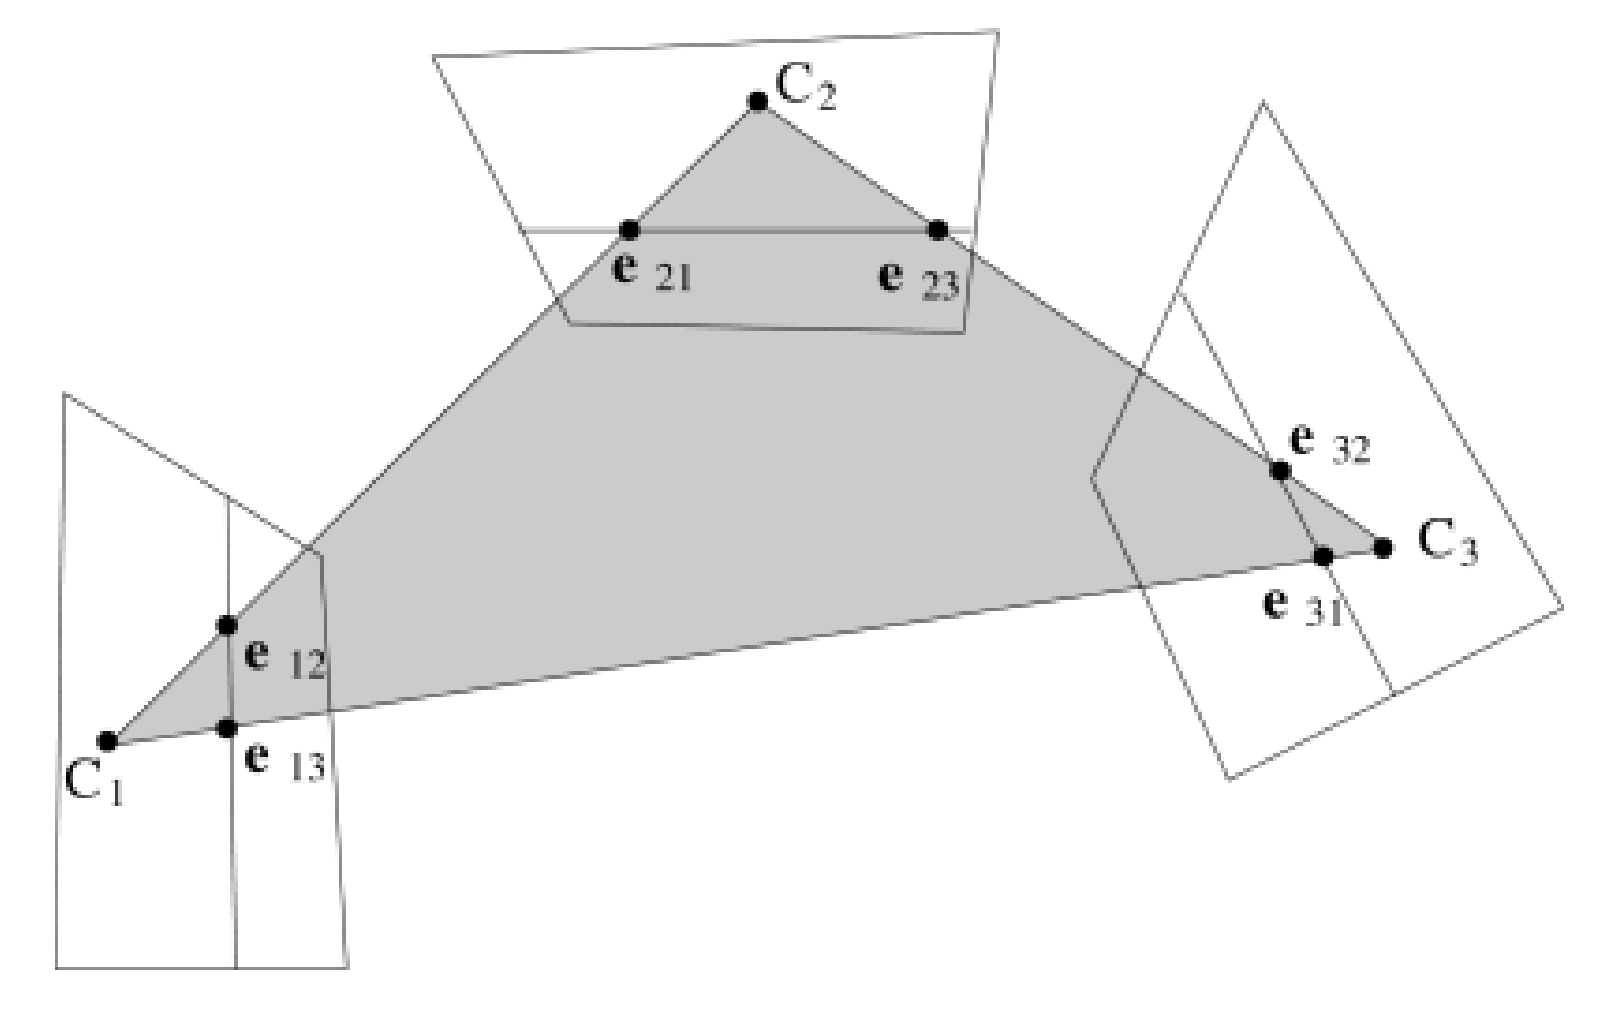
\includegraphics[width=0.7\textwidth]{figures/multiview_geometry.png}
% 	\caption{多视几何示例}
% 	\label{fig:multiview_geometry}
% \end{figure}

\par 在基于RGB-D 相机的三维重建中,RGB-D相机提供了额外的深度信息,这极大地简化了位姿估计
和三维重建的问题。利用深度信息,可以直接获得初始的三维点,然后通过优化位姿来提高重建的质量。
\section{kMaX-DeepLab模型}

% \subsection{背景}
\par kMaX-DeepLab\cite{kmeans_mask_transformer}是由Google联合约翰霍普金斯大学,在ECCV 2022的论文中提出的一种新的图像全景分割模型。
它分析了现有Transformer模型结构在图像识别任务上的弊端,提出使用kMaX解码器来替换Transformer中的解码器,不仅可以生成更合理的注意力图,而且还具有更好的性能。

\subsection{模型特征}

\par 如图\ref{fig:kmaxdeeplab}\cite{kmeans_mask_transformer}所示,kMaX-DeepLab 主要由三个组件构成,包含像素编码器(Pixel Encoder)、增强像素解码器(Enhanced Pixel Decoder)和 kMaX 解码器。

\begin{enumerate}
	\item 像素编码器使用任意的卷积神经网络(CNN)或Transformer主干,负责从输入图像中提取视觉特征,输出一个特征映射(Feature Maps),代表输入图像的高级语义信息。
	\item 增强像素解码器通过使用一系列的上采样层和卷积层,将像素编码器的特征映射上采样并恢复到输入图像的高分辨率。它输出一个特征映射,代表输入图像的像素级细节。
	\begin{figure}[htbp]
		\centering
		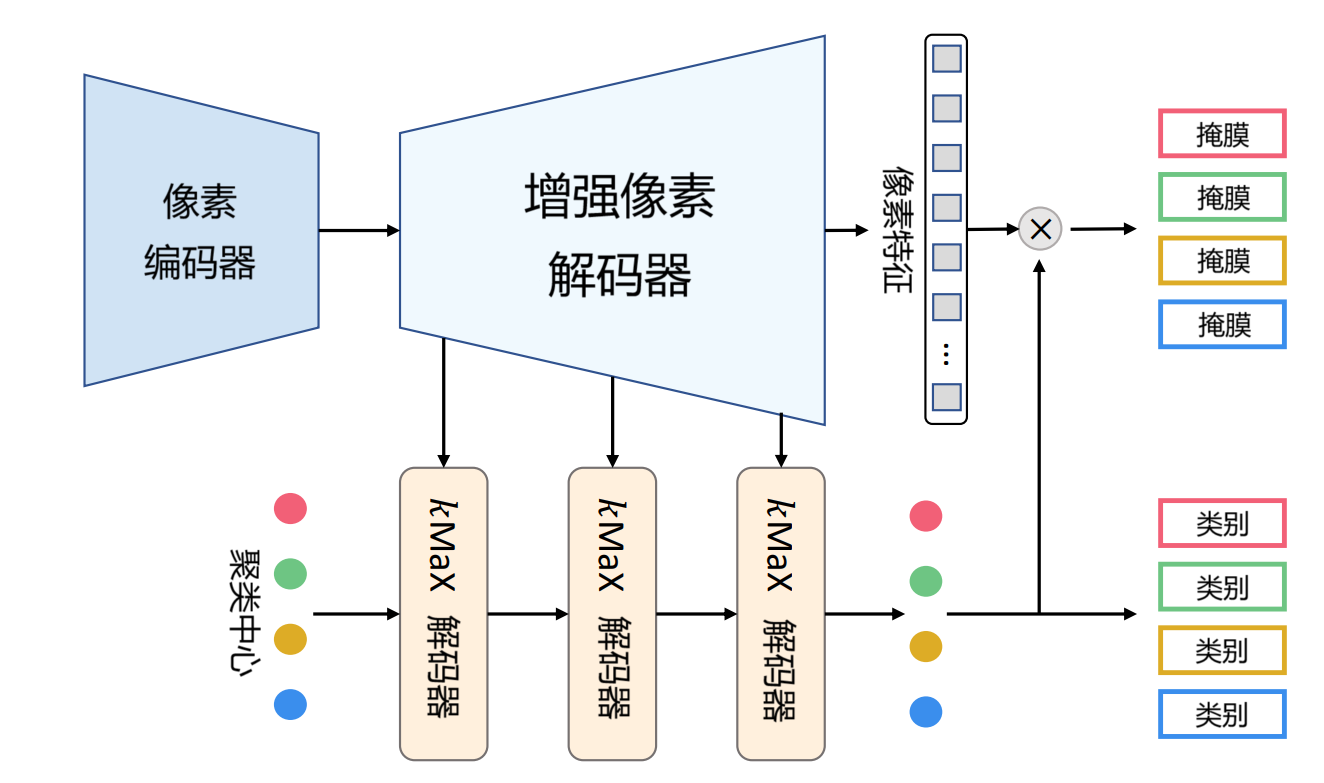
\includegraphics[width=0.9\textwidth]{figures/kmax_deeplab.png}
		\caption{kMaX-DeepLab 架构}
		\label{fig:kmaxdeeplab}
	\end{figure}
	\item kMaX 解码器负责将目标查询向量(如聚类中心)通过K-Means聚类转换成掩膜嵌入向量(Mask Embedding Vectors),如图\ref{fig:kmaxdecoder}\cite{kmeans_mask_transformer}所示。它会为每个目标查询向量输出一个掩膜嵌入向量,用来生成最终的分割掩膜。
	\begin{figure}[htbp]
		\centering
		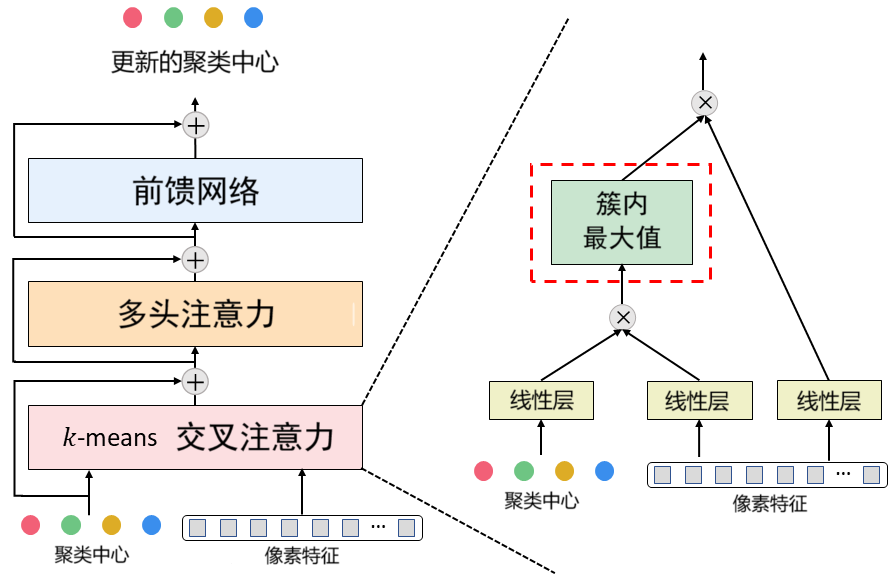
\includegraphics[width=0.9\textwidth]{figures/kmax_decoder.png}
		\caption{kMaX 解码器}
		\label{fig:kmaxdecoder}
	\end{figure}
\end{enumerate}

\subsection{注意力(Attention)机制}

\par 原始的 Mask Transformer(MaX-DeepLab)\cite{mask_transformer} 中的交叉注意力(Cross-Attention)机制使用空间(Spatial-Wise)Softmax 计算查询(Queries)和像素之间的相似度。这种方法有两个主要缺点:

\begin{enumerate}
	\item 计算量大,因为它需要对查询特征图(Object Queries)中的每个空间位置进行 Softmax 操作。
	\item 结果不准确,因为 Softmax 操作会平滑注意力的权重,使得区分重要性的特征变得模糊。
\end{enumerate}

\par kMaX-DeepLab 在 MaX-DeepLab\cite{mask_transformer} 和 CMT-DeepLab(Clustering Mask Transformer)\cite{cluster_mask_transformer} 像素簇聚类过程(图\ref{fig:cluster_mask_transformer})的基础上,提出了通过使用 K-Means 交叉注意力来解决这些问题,将 Mask Transformer\cite{mask_transformer}视为迭代执行聚类分配和聚类更新的过程。K-Means 交叉注意力首先将查询特征图聚类为固定数量的簇(Cluster)。然后通过找到最接近簇质心的关键特征图来计算每个簇的注意力权重。
这种方法比空间 Softmax 更高效,因为它只需要对整个查询特征图进行一次 K-Means 聚类操作。其次,这种方法也更准确,因为注意力权重不会被 Softmax 操作平滑。
因此,kMaX-DeepLab 的速度是原始 Mask Transformer 的3倍,在 Cityscapes 数据集上的准确率比原始 Mask Transformer 高出1.5\%。此外,kMaX-DeepLab 对噪声和离群值更具鲁棒性,训练效率更高,并且可以与其他注意力机制(如自注意力 Self-Attention)一起使用。

\begin{figure}[htb]
	\centering
	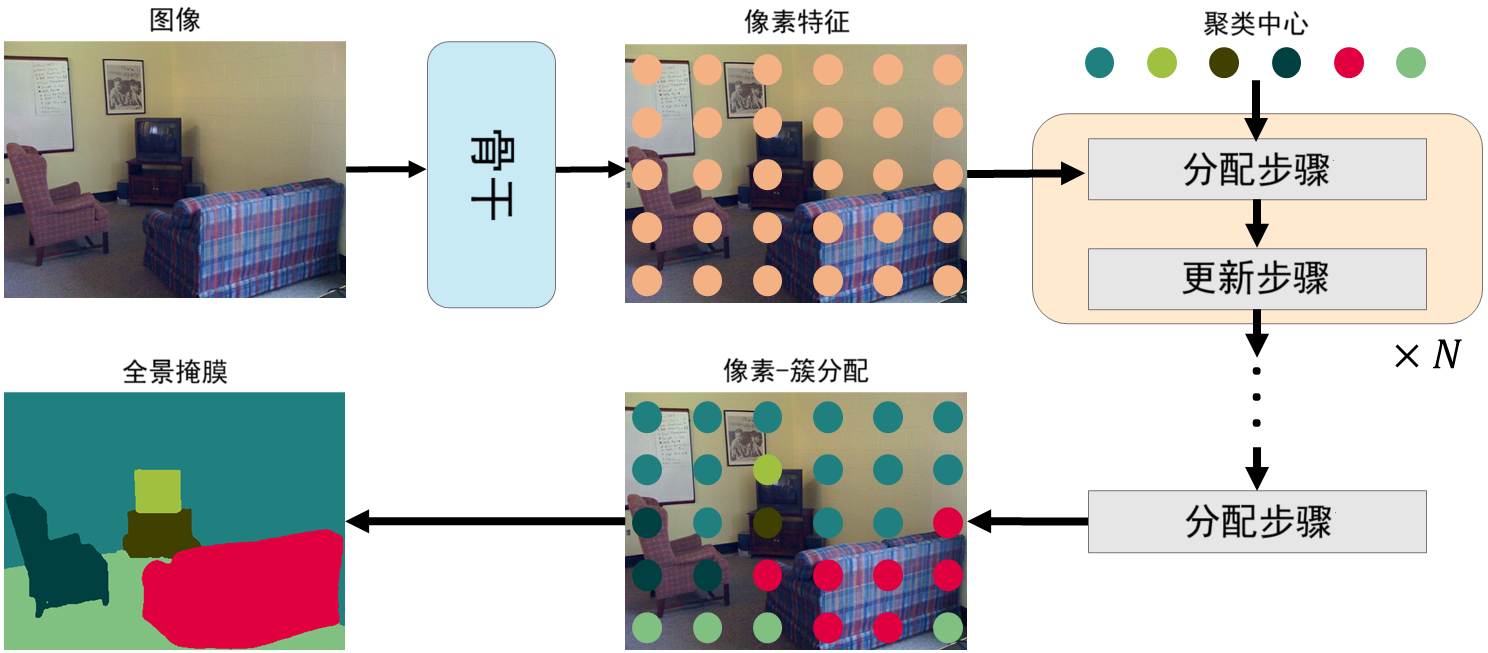
\includegraphics[width=0.9\textwidth]{figures/clustering_view_of_mask_transformer.png}
	\caption{CMT-DeepLab 像素簇聚类过程}
	\label{fig:cluster_mask_transformer}
	\note{注:CMT层根据特征相似度将像素分配给各个聚类中心,用于更新像素特征和聚类中心。经过多个 CMT 层后,获得精细的像素簇分配,产生最终的全景掩模。}
\end{figure}

% \subsection{模型效果}

% \par 如表\ref{seg model accuracy}所示,kMaX-DeepLab 在多种基准测试中都取得了最佳结果\cite{kmeans_mask_transformer}。在 COCO 数据集上的全景分割质量(panoptic quality,PQ)得分为58.0\%;在 Cityscapes 数据集上的 PQ 得分为68.4\%,精确率(average precision,AP) 得分为44.0\%,平均交并比(mean Intersection over Union,mIoU)
% 得分为83.5\%;在 ADE20K 数据集上的 PQ 得分为50.9\%,mIoU 得分为55.2\%。相对于先前的模型均产生了巨大的进步,
% 展示了基于 Transformer 的架构在全景分割方向的潜力。

% \begin{table}[htb]
% 	\centering
% 	\caption{全景分割模型测试结果}
% 	\label{seg model accuracy}
% 	\begin{tabular}{ccccc}
% 		\toprule
% 		Model              & backbone            & COCO $\text{PQ}^{\text{all}}$ & COCO $\text{PQ}^{\text{things}}$ & COCO $\text{PQ}^{\text{stuff}}$ \\
% 		\midrule
% 		kMaX-DeepLab       & ConvNeXt-L          & 58.1                          & 64.3                             & 48.8                            \\
% 		MaskFormer         & Swin-L (W12)        & 57.8                          & 64.2                             & 48.1                            \\
% 		Panoptic SegFormer & Swin-L (W7)         & 55.8                          & 61.7                             & 46.9                            \\
% 		CMT-DeepLab        & Axial-R104-RFN      & 55.3                          & 61.0                             & 46.6                            \\
% 		\toprule
% 		Model              & backbone            & Cityscapes PQ                 & ADE20K AP                        & ADE20K mIoU                     \\
% 		\midrule
% 		kMaX-DeepLab       & ConvNeXt-L          & 68.4                          & 44.0                             & 83.5                            \\
% 		Mask2Former        & Swin-L (W12)        & 66.6                          & 43.6                             & 82.9                            \\
% 		Axial-DeepLab      & Axial-ResNet-XL     & 64.4                          & 36.3                             & 80.6                            \\
% 		Panoptic-DeepLab   & SWideRNet-(1,1,4.5) & 66.4                          & 40.1                             & 82.2                            \\
% 		\bottomrule
% 	\end{tabular}
% \end{table}
\section{TSDF重建算法}

\par Truncated Signed Distance Function(TSDF)是实时三维重建技术的核心组成部分。此方法利用
深度传感器(如 RGB-D 相机)产生的数据来创建且更新 TSDF 模型,为三维重建提供基础。

\par TSDF 被设计为一种稀疏体素网格的数据结构,其中每一个体素都存储了相对于物体表面的有向距离信
息。该有向距离是以传感器的视角进行定义,对于被观察物体的表面,距离为0;对于物体表面的后
方,距离为正;对于物体表面的前方,距离为负,如图\ref{fig:tsdf_example}\cite{tsdf}所示。

\begin{figure}[htb]
	\centering
	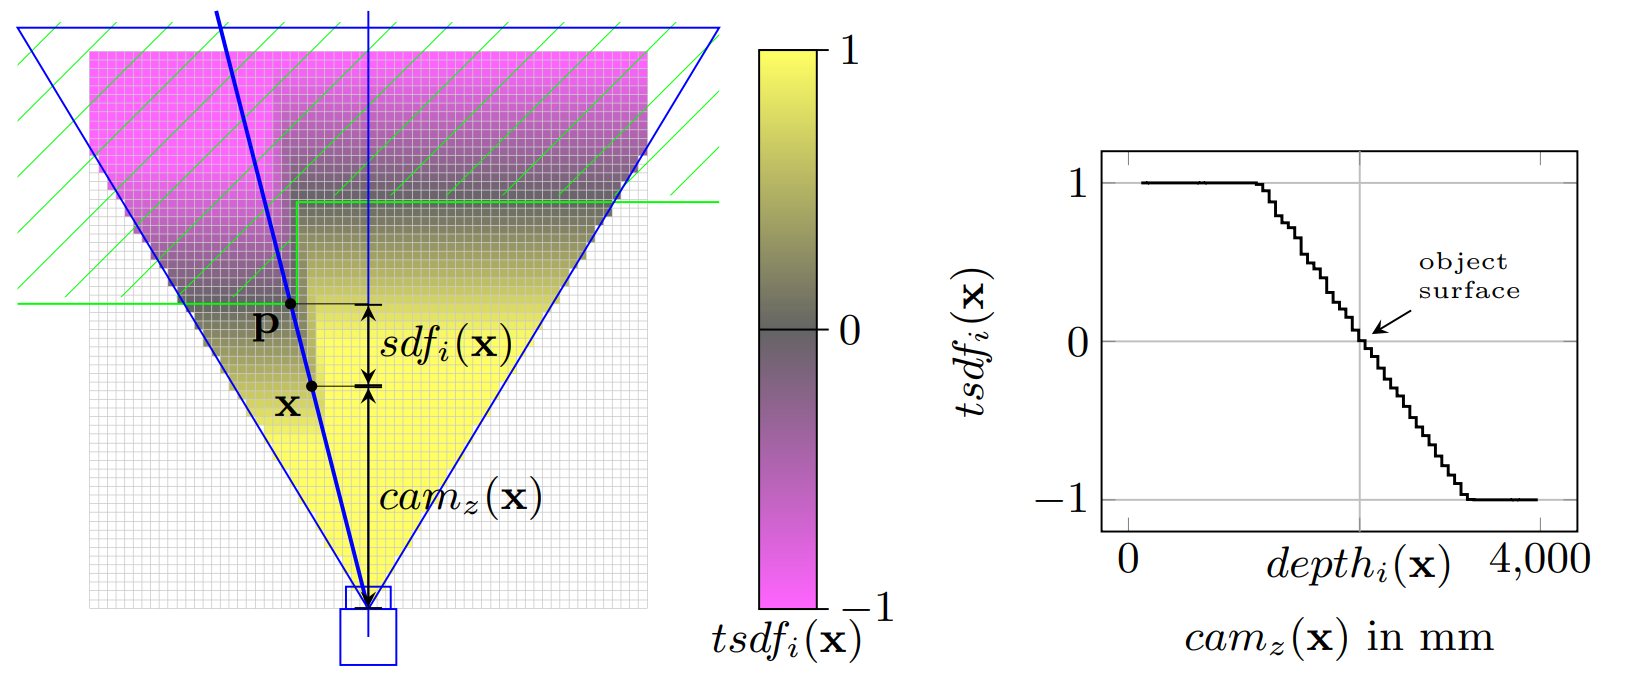
\includegraphics[width=0.9\textwidth]{figures/tsdf_exp.png}
	\caption{TSDF示例}
	\label{fig:tsdf_example}
	\note{注:固体物体:绿色;具有视场、光轴和光线的相机:蓝色;TSDF 网格:看不见的体素为白色,其他体素参见颜色条。体素 x 的有符号距离值由物体表面的深度和体素的相机距离 $cam_z(x)$ 确定。}
\end{figure}

\par 为了生成 TSDF,首先需要从 RGB-D 图像中获得深度信息。对于每一个像素,深度值可以被转
化为一个在三维空间中的点。这些点可以进一步被投影到一个预设的体素网格中,从而生成一个初步
的 TSDF 表示。以下公式描述了该过程:
\begin{equation}
	cam_z(x) = depth_i(pic(x))
\end{equation}
\begin{equation}
	x = K^{-1} pic(x) cam_z(x)
\end{equation}

\par 其中,$x$是世界坐标下的体素点,$pic(x)$是$x$对应的像素坐标,
$cam_z(x)$ 是$x$对应的像素的深度,即该像素所属物体到相机的距离,$K$ 是相机的内参矩阵。

\par 为了获取 TSDF 中每个体素的有向距离,需要计算每个体素中心点到物体表面的最
短距离。在理想情况下,这个距离是物体表面到体素中心的欧氏距离,但是为了方便计算,通常将其
近似为在相机视角下的直线距离。此外,还需要注意距离的截断处理。如果某个体素中心距离
物体表面的距离过大(超过预定的截断距离),则不考虑该体素对 TSDF 的贡献。以下公式描述了该
过程:
\begin{equation}
	sdf_i(x) = depth_i(pic(x)) - cam_z(x)
\end{equation}
\begin{equation}
	tsdf_i(x) = \max(-1, \min(1, \frac{sdf_i(x)}{t}))
\end{equation}

\par 其中,$sdf_i(x)$ 是体素中心点到物体表面的有向距离,$t$ 是预定的截断距离,
$tsdf_i(x)$ 是截断后的 TSDF 距离,$w_{\text{{voxel}}}$ 是体素的权重。

\par 在完成了 TSDF 的初始生成之后,如果输入新的 RGB-D 图像,就需要更新 TSDF。首先,根据相机位姿将新的 RGB-D 图像对齐到当前的 TSDF 模型中,然后
用新图像的数据更新 TSDF 的距离和权重:
\begin{equation}
	TSDF_i(x) = \frac{W_{i-1}(x)TSDF_{i-1}(x) + w_i(x)tsdf_i(x)}{W_{i-1}(x) + w_i(x)}
\end{equation}
\begin{equation}
	W_i(x) = W_{i-1}(x) + w_i(x)
\end{equation}

\par 其中,$W_{i-1}(x)$ 和 $TSDF_{i-1}(x)$ 是旧的 TSDF 体素权重和
距离,$w_i(x)$ 和 $TSDF_i(x)$ 是新的 TSDF 体素权重和距离。

\par TSDF 提供了一种有效的方法从 RGB-D 图像中生成和更新三维重建模型,且具有较好的
噪声抑制和缺失数据填充能力。然而,TSDF 算法也有其局限性,例如无法处理动态场景中的物体运动
,无法处理深度图像中的大范围空洞等。这些问题在后续的研究中也得到了一定程度的解决,例如动
态物体的问题可以通过引入运动分割算法来处理,深度图像中的空洞问题可以通过引入基于RGB图像
的深度补全算法来处理。
\section{并行计算与优化}

\subsection{GPU架构}

\paragraph{GPU简介}

\par GPU(Graphics Processing Unit)是一种高度并行结构,设计用于处理大规模的数据并行任务,
如图形渲染和科学计算。近年来也广泛应用于高性能计算和机器学习等领域。GPU由数百到数千个并行
处理核心组成,这些核心被组织在一个或多个流处理器(Streaming Multiprocessor,SM)中。
这些执行单元都是按照单指令多数据流方式运行的,即它们都执行相同的指令,但是对应于
不同的数据。因此,与CPU相比,GPU有着极高的并行处理能力,能够同时处理大量的并行任务。图\ref{fig:a100}和图\ref{fig:4090}展示了NVIDIA两款最新型号的GPU。

\begin{figure}[htb]
    \centering
    \begin{minipage}[t]{0.45\textwidth}
    \centering
    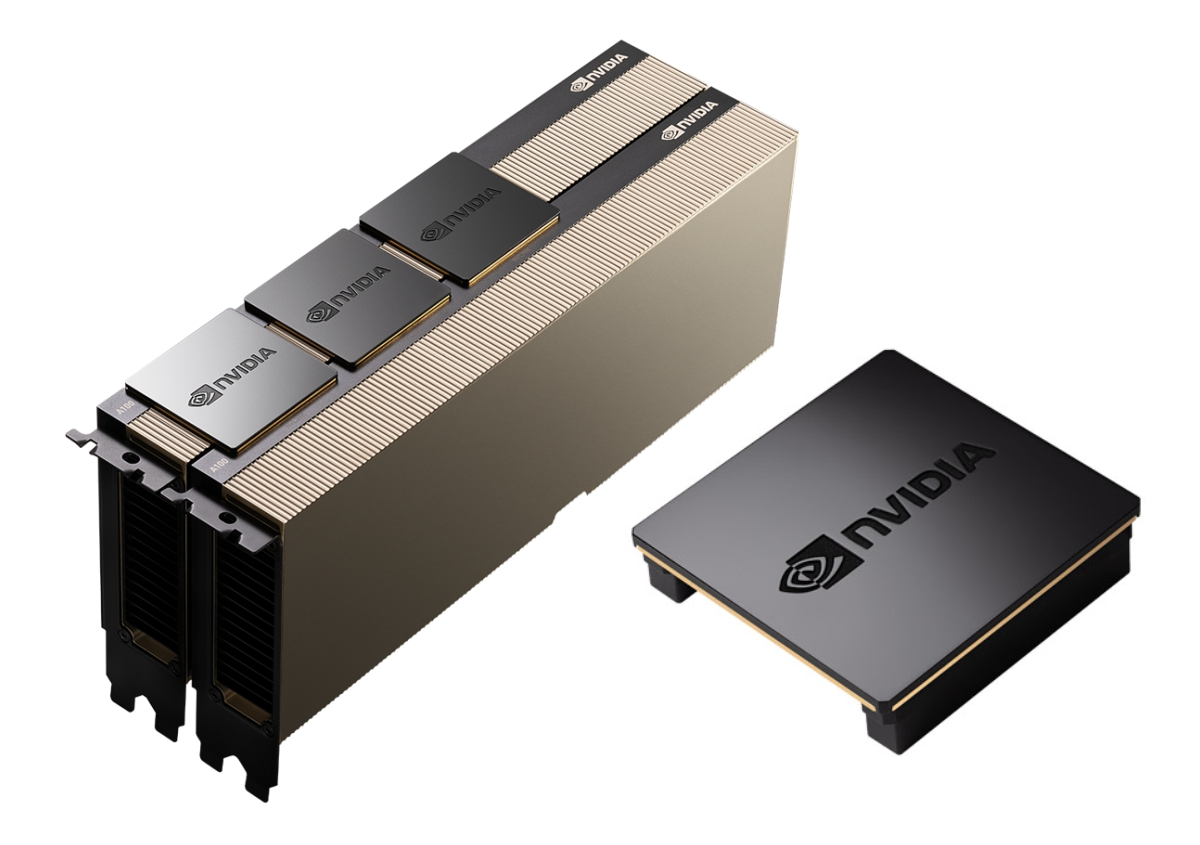
\includegraphics[height=4cm,keepaspectratio]{figures/a100.png}
    \caption{NVIDIA A100 Tensor Core GPU}
    \label{fig:a100}
    \end{minipage}
    % \hspace{1in}
    \begin{minipage}[t]{0.45\textwidth}
    \centering
    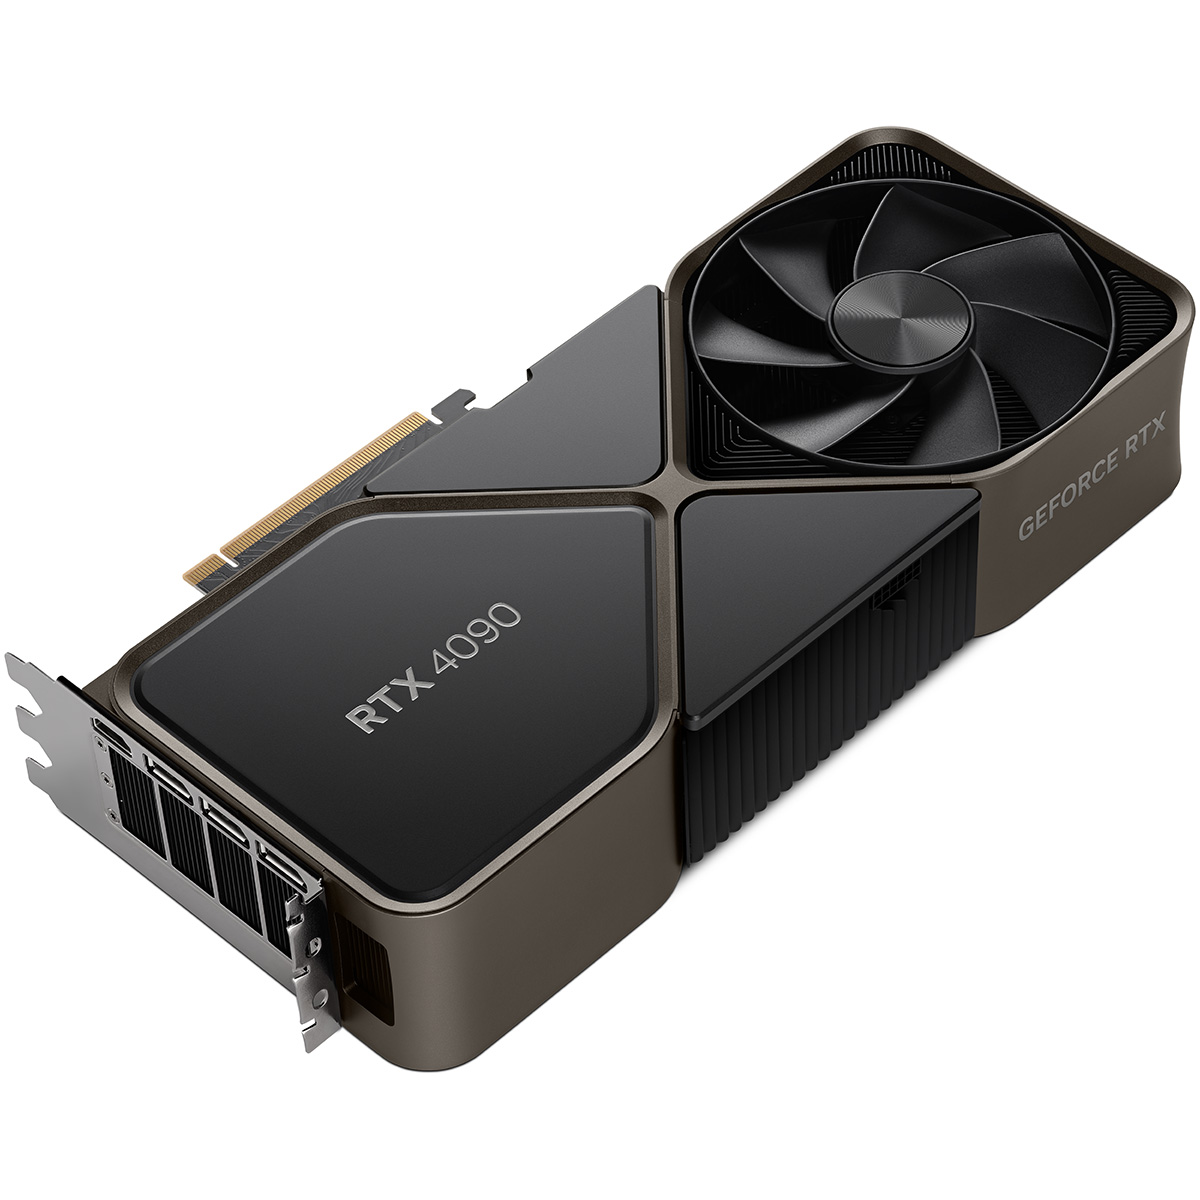
\includegraphics[height=4cm,keepaspectratio]{figures/4090.jpg}
    \caption{GeForce RTX 4090}
    \label{fig:4090}
    \end{minipage}
\end{figure}

\paragraph{GPU内存模型}

\par 如图\ref{fig:memory_hierarchy}\cite{nvidia_cuda}所示,GPU的内存模型是分层次的,包括全局内存(Global 
Memory)、共享内存(Shared Memory)、常量内存(Constant Memory)和纹理内存(Texture 
Memory)等。全局内存具有较大的存储容量,所有的线程都可以进行读写,但访问延迟较高。

\par GPU在运行时,首先从全局内存中读取数据,然后在各自的处理核心上执行一系列的指令,最后
将结果写回全局内存。共享内存提供给单个SM中的线程使用,具有较低的访问延迟,但容量较小。
常量内存和纹理内存主要用于读取操作,并且能通过缓存提高读取性能。另外,每个线程都拥有一些
私有的寄存器,用于存储临时的计算结果。当寄存器用完时,数据会溢出到本地内存。

\begin{figure}[htb]
    \centering
    \begin{minipage}[t]{0.55\textwidth}
    \centering
    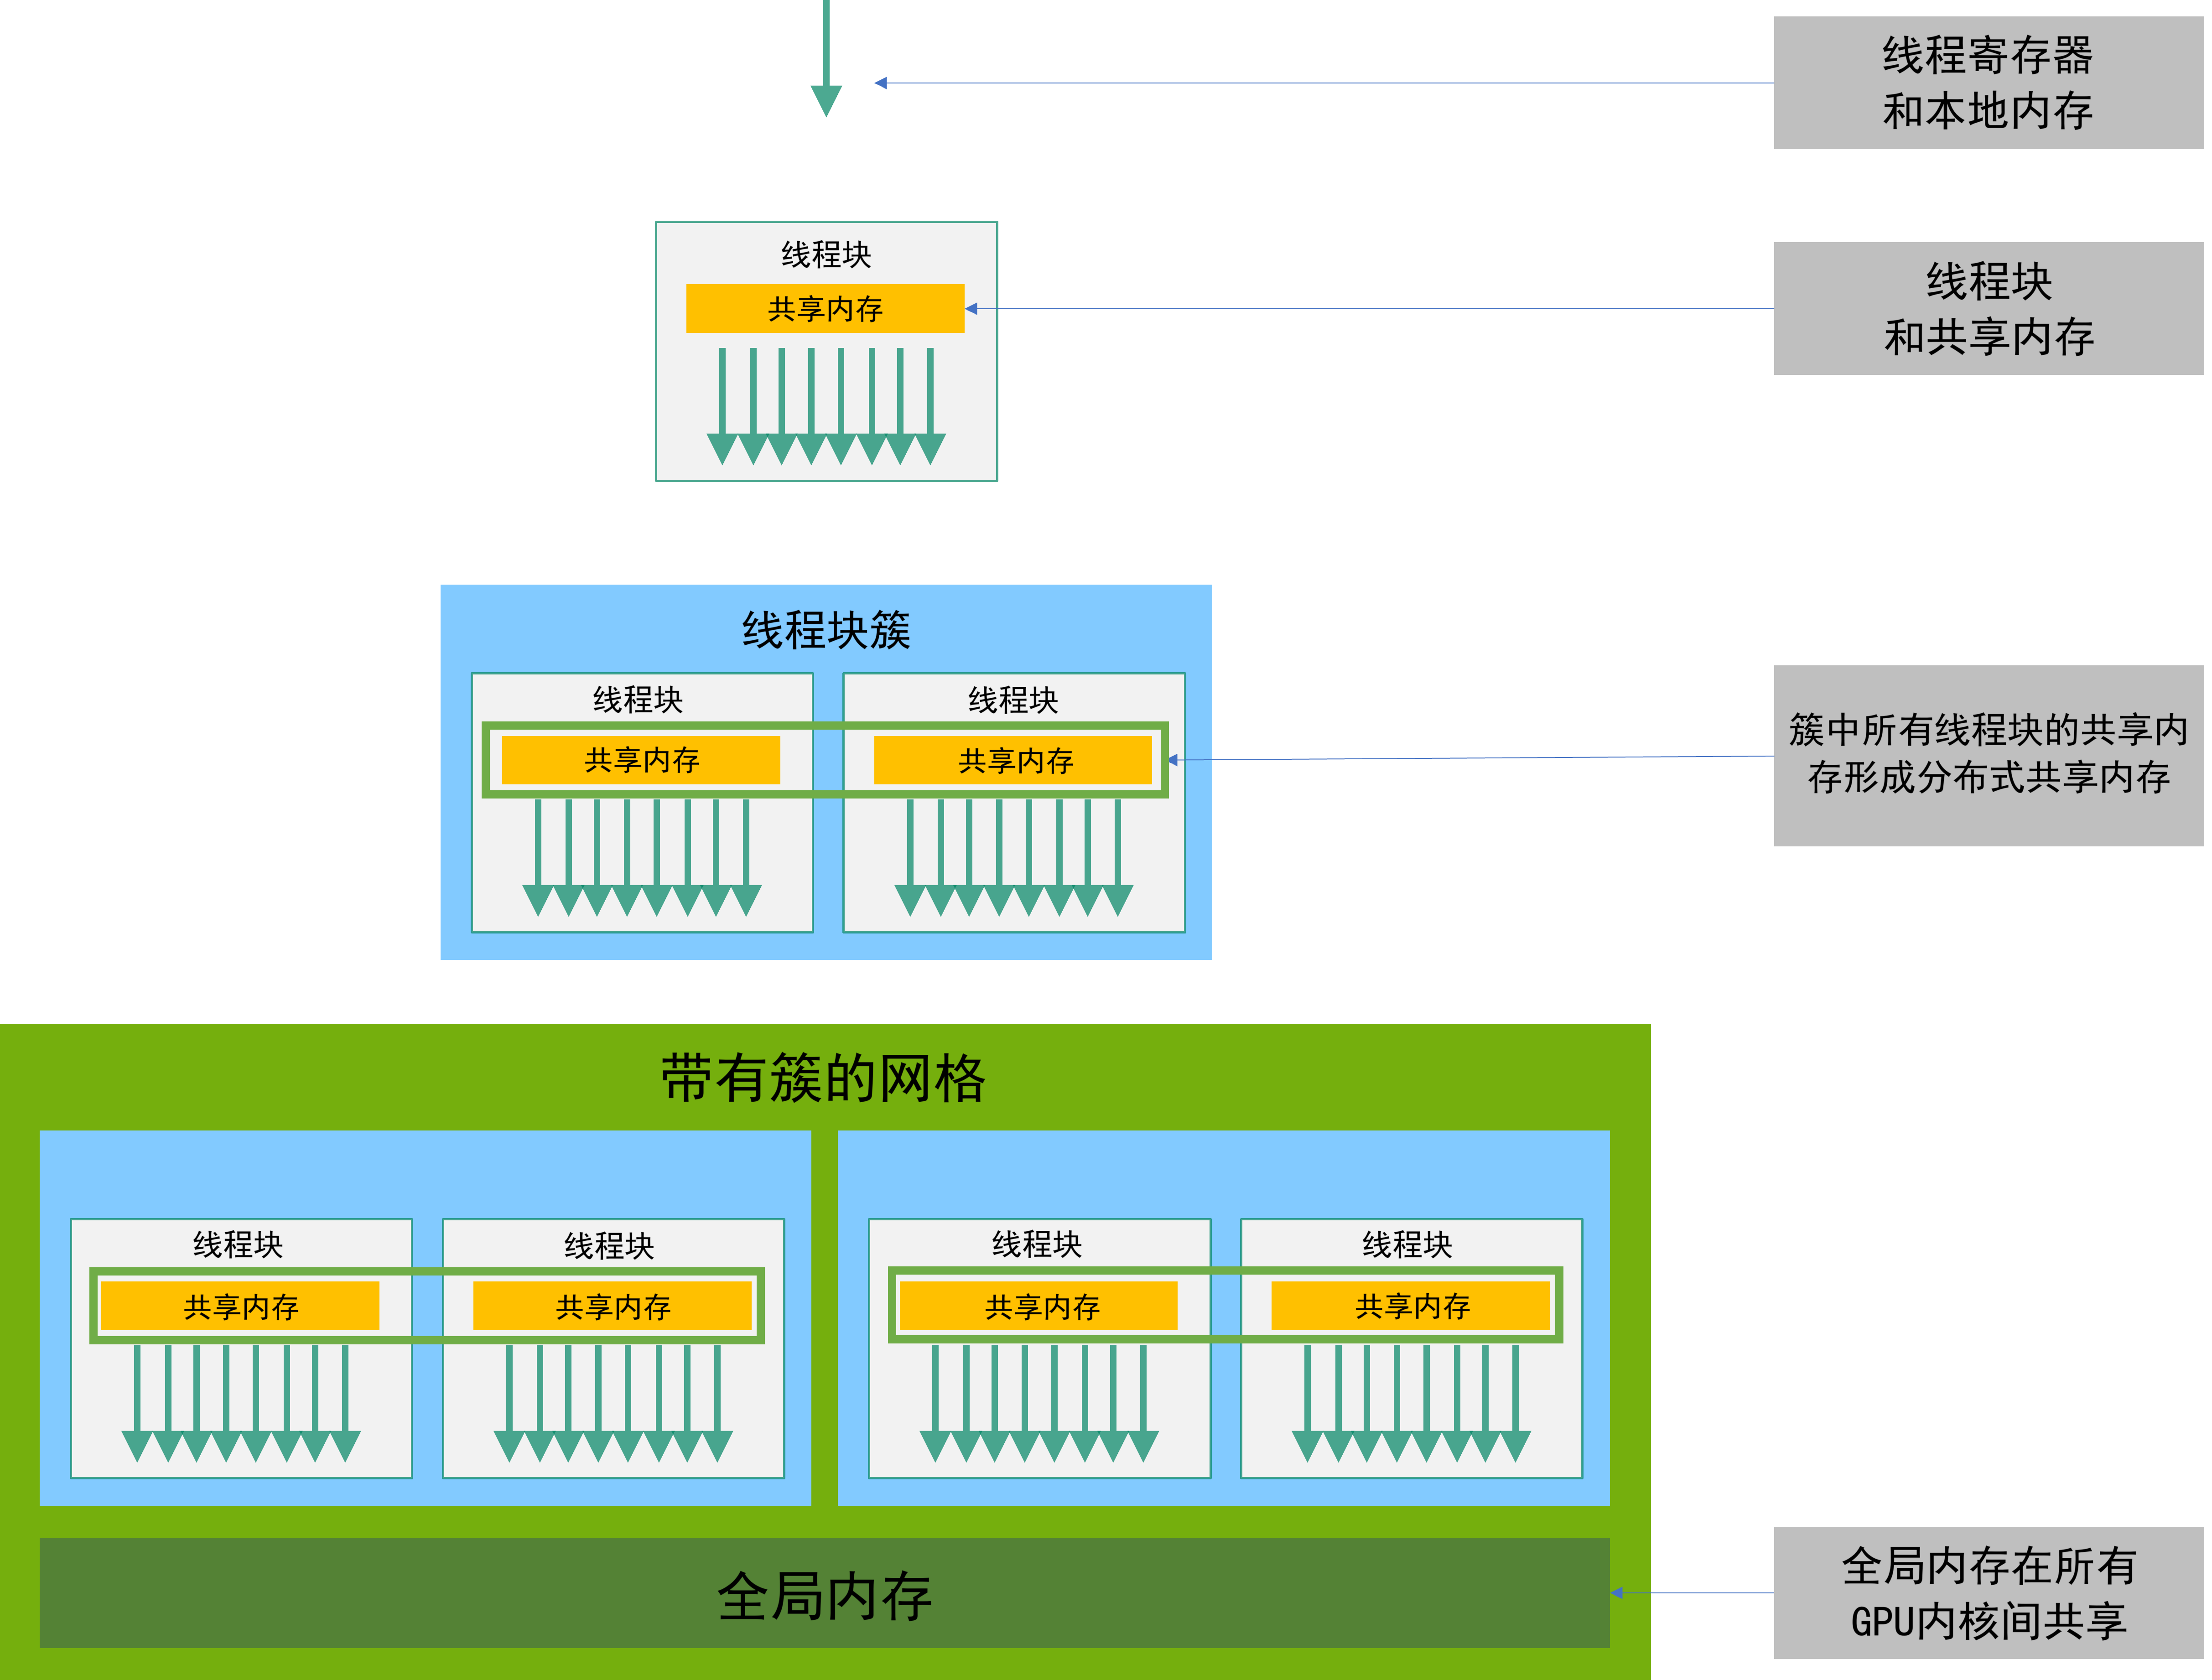
\includegraphics[width=0.9\textwidth]{figures/memory_hierarchy.png}
    \caption{GPU内存架构}
    \label{fig:memory_hierarchy}
    \note{注:GPU的分层内存模型,包括全局、共享、常量及纹理内存。}
    \end{minipage}
    % \hspace{1in}
    \begin{minipage}[t]{0.35\textwidth}
    \centering
    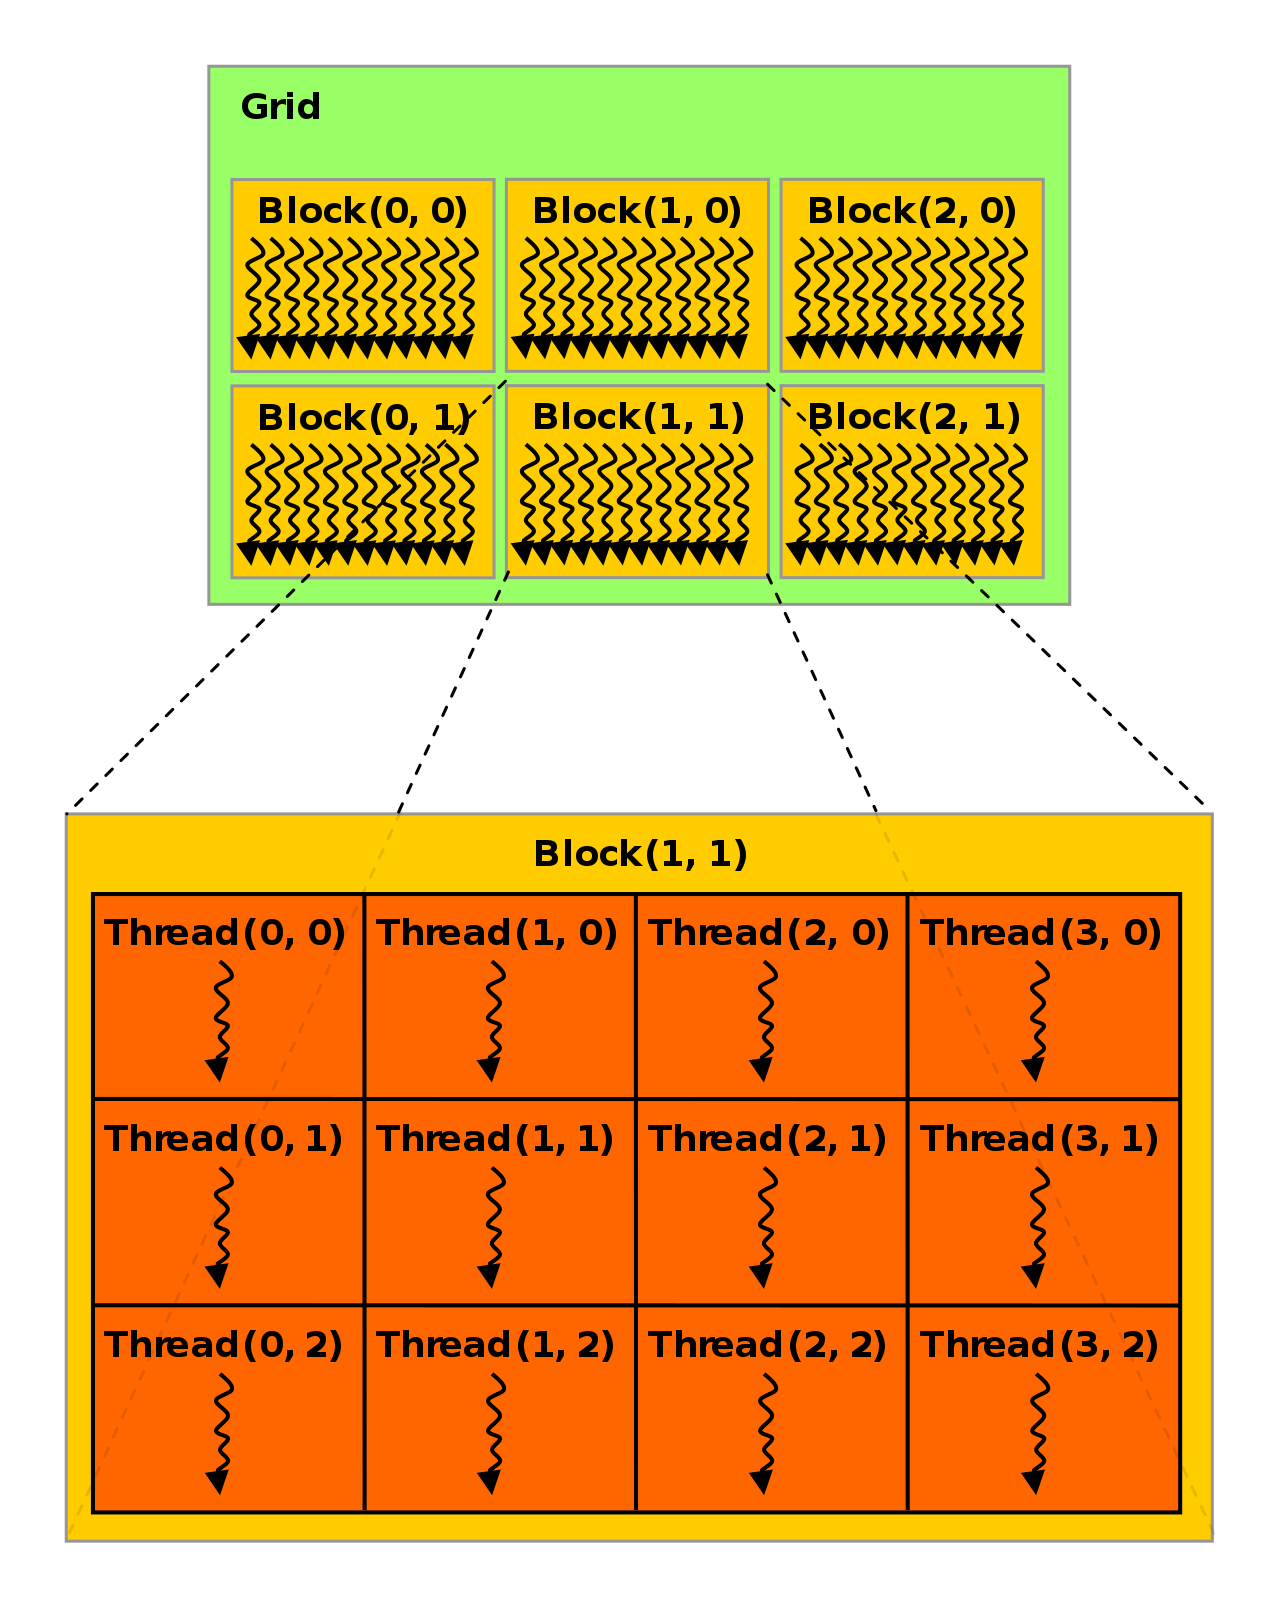
\includegraphics[width=0.9\textwidth]{figures/thread_block.png}
    \caption{GPU线程组织模型}
    \label{fig:block_thread}
    \note{注:GPU的层次化线程组织模型,包括线程、线程束、线程块和网格。}
    \end{minipage}
\end{figure}

\paragraph{GPU线程组织模型}

\par GPU采用如图\ref{fig:block_thread}\cite{nvidia_cuda}所示的层次化线程组织模型。基本单位是线程,每个
线程能够独立执行任务。在NVIDIA的架构中,32个线程组成一个线程束(Warp),这些线程同时执行
相同的指令,但是处理不同的数据。线程束进一步组织为线程块(Thread Block)。线程块内的线程
可以通过共享内存进行通信,协调它们的计算和内存访问。最后,线程块聚集在一起形成一个网格
(Grid),实现大规模的并行处理。

\subsection{CUDA编程}

\paragraph{CUDA简介}

\par CUDA(Compute Unified Device Architecture)是NVIDIA推出的并行计算平台和编程模型,
允许开发者利用NVIDIA的GPU进行通用计算。

\par CUDA提供了一系列的API,将GPU视为一个并行计算设备,允许开发者在C/C++中写并行代码,
称为内核(Kernel)。在CUDA编程模型中,程序员编写内核,指定并行线程的数量和配置,
并将内核提交给GPU执行。当线程维度为1时,线程数量和索引的计算方式如下:
\begin{equation}
    \begin{aligned}
    & \text{线程数量} = \text{blockDim.x} \times \text{gridDim.x} \\
    & \text{线程索引} = \text{blockIdx.x} \times \text{blockDim.x} + \text{threadIdx.x}
    \end{aligned}
\end{equation}

\par 此外,CUDA也支持各种高级特性,如动态并行、双精度浮点运算、原子操作和 CUDA 图等。

\paragraph{CUDA编程规范}

\par 在 CUDA 编程中,线程的组织模型与 GPU 硬件模型密切关联,这对于实时三维重建及语义分割
系统极其重要。开发过程中需要以线程束、线程块和网格的形式来管理和调度线程,以便充分利用 GPU 
的硬件特性。例如,为了避免全局内存访问的延迟,可以在共享内存中存储重建和分割过程中频繁使用的
数据,然后将其分发到各个线程\cite{nvidia_cuda}。在编程过程中,需要确保线程束内的所有线程
都执行相同的指令,以免影响系统性能。对线程束和线程块的工作方式的理解可以更有效地组织和调度线
程,避免在三维重建及语义分割过程中产生的同步和通信开销。此外,还需要考虑如何在全局内存、共享
内存和寄存器之间高效地传输和存储三维重建及语义分割所需的数据。
\section{图形渲染技术}

\subsection{OpenGL图形库}

\par OpenGL(Open Graphics Library)是一个由美国硅图技术公司开发,现由Khronos Group维护的跨语言、跨平台的专业图形库,被广泛应用于计算机辅助设计(Computer Aided Design,CAD)、虚拟现实、科学可视化、游戏引擎和飞机模拟等领域。

\par OpenGL的设计基于一个状态机,其内部定义了近300个用于绘制不同场景的函数,其中的大部分函数用于更改内部状态,而不是直接操作图形数据。
它支持多种渲染技术,包括纹理映射、阴影生成、抗锯齿、透明度、光照模型等。

\par OpenGL主要特点是跨平台性和扩展性,可以运行在各种操作系统(如Windows、Mac OS、Linux等)和硬件平台上。由于OpenGL是一个开放标准,因此可以被各种硬件制造商和开发者自由地使用和扩展。

\par 此外,OpenGL的另一个显著特点是强大的性能,随着GPU等计算机图形硬件的不断发展,可以更高效地渲染复杂的三维场景,以及支持新的渲染技术和效果。

\subsection{渲染管线}
\par 图形渲染管线\cite{OpenGL_graphics_system}是硬件和软件之间的抽象,输入需要渲染的三维物体的相关描述信息(如顶点坐标、顶点颜色、顶点纹理等),
经过一系列变换与渲染的过程,在计算机屏幕输出二维图像。如图\ref{fig:glpipeline}所示,主要分为两个阶段:几何阶段和光栅化阶段。

\begin{figure}[htb]
	\centering
	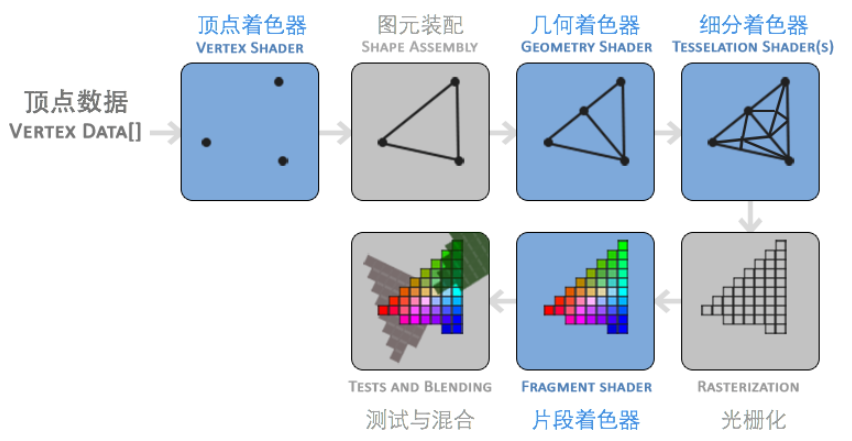
\includegraphics[width=0.9\textwidth]{figures/opengl_pipeline.png}
	\caption{OpenGL渲染管线}
	\label{fig:glpipeline}
	\note{注:OpenGL渲染管线的两个主要阶段:几何阶段和光栅化阶段。}
\end{figure}

\paragraph{几何阶段}

\par 该阶段负责处理所有关于几何图形(如顶点和线)的数据。主要包括以下步骤:

\subparagraph{顶点着色器(Vertex Shader)}
\par 这是GPU上运行的第一个程序,负责处理三维空间中的顶点数据。它的任务包括变换坐标,计算光照和颜色等。

\subparagraph{图元装配(Primitive Assembly)}
\par 顶点着色器处理完顶点数据后,将这些顶点组装成几何图元,如点、线、三角形等。

\subparagraph{几何着色器(Geometry Shader)}
\par 可选阶段,可以在此创建新的顶点或者丢弃某些几何图元。

\subparagraph{裁剪(Clipping)}
\par 丢弃不会出现在最终屏幕上的几何图元。

\paragraph{光栅化阶段}
\par 该阶段负责将几何图形转换为像素图像,主要包括以下步骤:

\subparagraph{光栅化(Rasterization)}
\par 将裁剪后的几何图形转换为像素图像,得到的结果称为片元(Fragment)。

\subparagraph{片元着色器(Fragment Shader)}
\par 将每个片元通过片元着色器进行处理,计算最终的颜色和其他属性。

\subparagraph{Alpha测试和混合(Alpha Testing and Blending)}
\par 最后,检查每个片元的透明度并混合在一起,得到最终的像素颜色。

\section{本章小结}
\par 本章详细阐述了基于 RGB-D 相机的实时三维重建及语义分割系统的关键技术。
首先,介绍了基于对极几何的相机位姿估计方法,为后续的三维重建提供了基本的空间信息。
然后,详述了kMaX-DeepLab模型的特性和注意力机制,实现了对RGB图像的高效语义分割。
接着,讨论了TSDF算法的应用,以及如何利用GPU架构与CUDA编程进行实时点云生成和语义融合。
最后,对OpenGL的主要特点和渲染管线进行了深入研究,以满足系统的可视化需求。
这些关键技术为系统的实现奠定了理论与技术基础。


